\chapter{Dijkstra - Algorithmus}

\section{Erklärung}

\subsection{Das Shortest-Path Problem}
Das Shortest-Path Problem ist in der Literatur manchmal auch unter dem Namen Single-Source Shortest Path Problem zu finden. 
Es behandelt die Frage, wie man in einem Graphen ausgehend von einem gegebenen Anfangsknoten s (engl. Source) zu jedem anderen Knoten des Graphen den kürzesten Pfad findet \footnote{OTTMANN, Thomas; WIDMAYER Peter: Algorithmen und Datenstrukturen, Reihe Informatik Bd. 70, Mannheim: BI-Wissenschaftsverlag, 1990, S. 572, Z. 19-20}. Mit kurz ist hierbei nicht die Länge gemeint, sondern die Minimierung der Kantenkosten. Im Allgemeinen ist mit Länge nicht die tatsächliche Länge gemeint, sondern die Pfadkosten.


\subsection{Zur Eingabe}
Die Eingabe besteht stets aus gerichteten Graphen. Hierbei muss jedoch angemerkt werden, dass sich jeder ungerichtete Graph leicht in einen gerichteten Graph umwandeln lässt, indem für jede Kante \{u,v\} die Kanten (u,v) und (v,u) mit gleichen Kosten eingeführt werden.\footnote{Vorlesungsskript Algorithmendesign, Prof.Dr.Heinz Schmitz, Stand 6. April 2015, S.133 Z.8-13} Somit findet der Dijkstra-Algorithmus auch für ungerichtete Graphen Anwendung, solange sie vorher in einen Digraphen überführt werden. 

\parindent0pt Zudem wird davon ausgegangen, dass die Kantenkosten nicht negativ sind.

\subsection{Das Optimalitätsprinzip}
Dem Dijkstra-Algorithmus liegt das Optimalitätsprinzip zugrunde:

\parindent0pt Für jeden kürzesten Pfad p=(v{\tiny 0},v{\tiny 1},...,v{\tiny k}) von v{\tiny 0} nach v{\tiny k} ist jeder Teilweg p'=(v{\tiny i}, ..., v{\tiny j}) mit $0 \le i < j \le k$ ein kürzester Weg von v{\tiny i} nach v{\tiny j}.

\parindent0pt Das bedeutet kurz gesagt, dass  für alle möglichen Teilpfade angenommen wird, dass sie optimal sind.
Dass diese Annahme stimmt, lässt sich mittels Widerspruchbeweis nachweisen: 

\parindent0pt Wird vom Gegenteil ausgegangen, nämlich dem Fall, dass neben dem Pfad p' von v{\tiny i} nach v{\tiny j} ein anderer, kürzerer Pfad p'' von v{\tiny i }nach v{\tiny j} existiert, Dann müsste p' durch p'' ersetzen werden (denn p'' ist kürzer). Damit würde sich auch der Gesamtpfad von v{\tiny 0} nach v{\tiny k} verkürzen. Da unser Pfad p von v{\tiny 0} nach v{\tiny k} bereits der kürzeste war, ist das  ein Widerspruch. \footnote{OTTMANN, Thomas; WIDMAYER Peter: Algorithmen und Datenstrukturen, Reihe Informatik Bd. 70, Mannheim: BI-Wissenschaftsverlag, 1990, S.573, Z.1-5}


\subsection{Funktionsweise des Algorithmus}
Auf welche Weise kann eine optimale Lösung gefunden werden?
Die Grundidee besteht darin, für jeden Knoten die Pfadkosten zu schätzen und die bestehende Lösungsmenge mit dem Knoten zu erweitern, welcher den geringsten Schätzwert aufweist. 

\parindent0pt Diese Arbeitsweise entspricht dem Greedy-Entwurfsmuster (engl. gierig): Nach einem Auswahlkriterium (die sogenannte Greedy-Regel) wird aus einer Menge das Element zur Erweiterung der Lösung gewählt, das den meisten Nutzen verspricht. In diesem Fall ist die Greedy-Regel das Verlangen nach dem kleinsten Schätzwert.
Auf das Greedy-Prinzip wird in dieser Arbeit jedoch nicht tiefergehend eingegangen.

\parindent0pt Dijkstra geht bei seinem Algorithmus folgendermaßen vor: Er unterteilt die Knoten des Graphen zunächst einmal in drei Gruppen: Die Knoten, deren Schätzwert bereits feststehen ("black nodes"\footnote{DIJKSTRA Edsger W., FEIJEN W.H.J.: A Method of Programming,Cornwall: Addison-Wesley Publishing Company,1988, S.107 Z.24}), deren Nachfolger ("grey nodes")\footnote{vergl. Ebd., S.108, Z.2-3} sowie unerreichbare Knoten, deren Schätzwerte gänzlich unbekannt sind ("white nodes" \footnote{vergl. Ebd., S.108, Z.3}).

\begin{figure}[h]
\centering
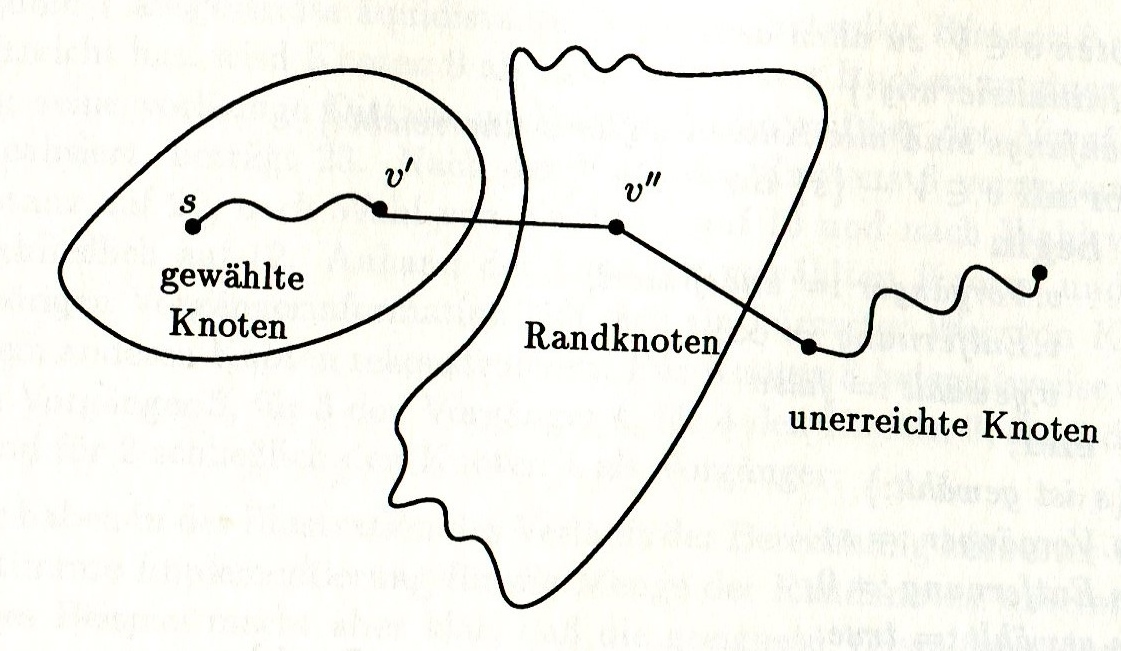
\includegraphics[width = 8cm]{./chapters/knotentypen.jpg}
\caption{Knotentypen {\tiny (Quelle: OTTMANN, Thomas; WIDMAYER Peter: Algorithmen und Datenstrukturen, Reihe Informatik Bd. 70, Mannheim: BI-Wissenschaftsverlag, 1990, S.573 Abb. 8.19)} }
\label{a1}
\end{figure}


\parindent0pt Des besseren Leseflusses wegen, werden die "black nodes", "white nodes" und "grey nodes" in der deutschen Übersetzung verwendet.
 Wenn keine grauen Knoten vorhanden sind, lässt sich die Lösungsmenge nicht erweitern. 

\parindent0pt Ansonsten muss aus den grauen Knoten einer ausgewählt werden, der schwarz werden soll, d.h. der Knoten, mit dem die Lösungsmenge erweitert wird. Alle vorherigen Pfade bestehen dabei ausschließlich aus schwarzen Knoten, d.h. Knoten die mit endgültig festgelegten Schätzwerten der Lösungsmenge bereits hinzugefügt wurden.

\parindent0pt Um zu bestimmen, welcher graue Knoten gewählt wird, müssen die Kosten seines speziellen Pfades bestimmt werden \footnote{vergl. Ebd., S.108,Z.8-12}, d.h. den Pfad ausgehend vom Startknoten s bis hin zur Kante vom letzten schwarzen Knoten zum aktuellen grauen Knoten. Der Knoten, dessen spezieller Pfad am kostengünstigsten ist, wird in die Menge der schwarzen Knoten aufgenommen und aus der Menge der grauen entfernt. Ist dieser Schritt vollzogen, müssen noch seine Nachfolger behandelt werden. Dabei gibt es für jeden Nachfolger drei Möglichkeiten:

\parindent0pt Fall 1: Der Nachfolger ist weiß, d.h. er hat noch keinen Schätzwert. Dann wird dieser jetzt bestimmt und der Knoten wird grau.

\parindent0pt Fall 2: Der Nachfolger ist grau. Dann muss verglichen werden, ob der aktuelle Schätzwert geringer ist als der vorherige, und wenn dies zutrifft, wird der Wert entsprechend aktualisiert. Das ist immer dann der Fall, wenn ein kostengünstigerer Pfad für den entsprechenden Knoten gefunden wurde.

\parindent0pt Fall 3: Der Nachfolger ist schwarz. Dann steht sein Schätzwert bereits fest und er kann ignoriert werden.

\subsection{Realisierung}
Um dies umzusetzen, geht Dijkstra folgendermaßen vor: In einem Array werden die Farben der Knoten gespeichert. Ein weiteres Array dient der Speicherung der Schätzwerte. 

\parindent0pt Da der Knoten mit minimalen Pfadkosten nur aus den grauen gewählt wird, ist es sinnvoll, ein Feld für diese anzulegen, wobei eine Variable, die zugleich als Zeiger dient, deren Anzahl speichert.

\parindent0pt Des weiteren werden zu jedem Knoten deren unmittelbare Vorgänger gespeichert, sodass sich der vollständige Pfad zu jedem Knoten zurückverfolgen lässt (Rekursion).

\parindent0pt Eingegeben wird ein Graph zusammen mit Startknoten s und Zielknoten v. Ist v nicht von s aus erreichbar, sind die zurückgegeben Pfadkosten 0. Ansonsten wird die Länge zurückgegeben.

\parindent0pt Das konkrete Vorgehen sieht nun folgendermaßen aus: \\

\parindent0pt \underline{1. Initialisierung:} Alle Knoten werden auf weiß gesetzt, der Startknoten s wird grau.

\parindent0pt \underline{2. Erweiterung:} Der Knoten mit minimalem Schätzwert wird aus der Menge der grauen Knoten ausgewählt und herausgenommen. Er wird auf schwarz gesetzt, sein Schätzwert ist nun endgültig.

\parindent0pt \underline{3. Aktualisierung: }Nun werden alle Nachfolger betrachtet. Deren Schätzwerte werden gegebenenfalls aktualisiert, wenn deren Pfadkosten nun geringer sind. \\ 

\parindent0pt Der Algorithmus terminiert, wenn alle grauen Knoten abgearbeitet sind bzw. wenn der letzte Knoten schwarz ist. \\

Natürlich kann auch eine Alternative zu Dijkstras Vorgehen mit Speicherung der Farbstufen gewählt werden. Der Algorithmus kann auch umsetzen werden, indem die Schätzwerte in einem Array gespeichert werden und die Knoten in einer Menge Q. Am Anfang werden alle Schätzwerte auf undefiniert gesetzt, das entspricht den weißen Knoten. Die Knoten aus Q, deren Schätzwert feststeht, werden aus Q entfernt, d.h. die schwarzen Knoten entsprechen der Differenz zwischen V und Q (V/Q). Alle übrigen Knoten in der Menge sind mit den grauen Knoten gleichzusetzen, welche jedoch erst vorläufige Schätzwerte darstellen. Das grundlegende Vorgehen ist bei einer solchen Implementierung gleich. 



\section{Komplexität}

\subsection{Ursprüngliche Implementierung}

Der folgende Abschnitt bezieht sich direkt auf Dijkstras eigene Implementierung, die von Ottman und Widmayer aufgegriffen wurde /footnote{Vgl. }
Das Initialisieren der Arrays benötigt jeweils $O(m)$ Schritte, wobei m die Kardinalität der Knotenmenge des Graphen ist.
Die äußere Schleife arbeitet alle grauen Knoten ab und benötigt daher ebenfalls $O(m)$ Schritte. Das Bestimmen des Minimums braucht ebenfalls $O(m)$ Schritte.
Das Aktualisieren der Nachfolger benötigt $O(deg(v))$ Schritte, also die Anzahl der ausgehenden Kanten des Knotens v, die maximal k beträgt (Gesamtzahl Kanten). Da in jedem Fall gilt, dass k &<& m (jede Kante mündet in zwei Knoten), kann dies vernachlässt werden, ebenso wie die übrigen verwendeten Operationen, die konstant sind.
Insgesamt ergibt sich so eine Laufzeit von $O(m^{2})$,\footnote{OTTMANN, Thomas; WIDMAYER Peter: Algorithmen und Datenstrukturen, Reihe Informatik Bd. 70, Mannheim: BI-Wissenschaftsverlag, 1990,S.576,Z.13} da m mal das Minimum in $O(m)$ bestimmt wird.
Das ist bei dünnen Graphen, also Graphen mit wenig Kanten im Verhältnis zur Knotenzahl sehr ineffizient. Im Vergleich zu günstigeren Implementierungen ist die Laufzeit recht hoch.

\subsection{Implementierung mit Heap}
Die von Dijkstra vorgeschlagene Implementierung lässt sich verbessern, indem zur Speicherung der grauen Knoten ein Heap eingesetzt wird, denn in einem Heap lässt sich das Bestimmen des Minimums und dessen Entfernen in $O(log m)$ bestimmen.

\parindent0pt Das Einfügen eines Elementes beträgt ebenfalls $O(log m)$ Schritte.

\parindent0pt Zwar ist das gezielte Löschen von Knoten mit veralteten Werten nicht möglich, sodass eventuell mehrere Knoten mit gleichen Werten existieren, dies ist jedoch nicht weiter schlimm, "wenn man für jeden Knoten nur die erste Entnahme dieses Knotens aus dem Heap beachtet und alle weiteren ignoriert".\footnote{vergl. Ebd.S.576 Z.29-31} Damit dies funktioniert, muss  gespeichert werden, welche Knoten bereits betrachtet wurden und welche nicht.

\parindent0pt Jede Kante erhält maximal einen Eintrag im Heap, also enthält dieser nie mehr als k Kanten. Damit kostet das Einfügen $k*log(m)$ Rechenschritte, ebenso wie das Entfernen. Somit ergibt sich für die Implementierung mit Heap eine Laufzeit von $O(k*log(m))$\footnote{vergl. Ebd., S. 576 Z.36}, was den Algorithmus bei dünnen Graphen sehr effizient macht.
Bei sehr dichten Graphen, also Graphen mit vielen Kanten,  mit $k = \Omega (m^{2})$ schneidet der ursprüngliche Dijkstra dagegen besser ab.

\parindent0pt Durch die Verwendung eines speziellen Heaps, dem Fibonacci-Heap, lässt sich eine Laufzeit von $O(k + m * log(m))$ \footnote{vergl. Ebd., S.577 Z.10} erreichen, wodurch die Implementierung mit einem Heap auch bei dichten Graphen effizienter ist.


\section{Implementierung}

\Das folgende Codebeispiel bezieht sich auf die bereits beschriebene Implementierung mit Heap /footnote{Vgl. Abs. 3.2.2, "Implementierung mit Heap"}

\lstset{language=Python}
\begin{lstlisting}
from heapq import heappush, heappop

def dijkstra_pq(G,s):
    m = len(G)                              #O(1)
    pq = []       #priority queue           #O(1)
    d = [None]*m  #kosten                   #O(m)
    p = [None]*m  #vorgaenger		       #O(m)
    d[s] = 0                                #O(1)
    heappush(pq, (0,s))                     #O(m)
    while pq:                               #O(m)
        (_,v) = heappop(pq)                 #O(log m)
        for u in G[v]:                      #O(deg(v)) --> O(k)  
            alt = d[v] + G[v][u]            #O(1)
            if d[u]== None or alt < d[u]:   #O(1)
                d[u] = alt		            #O(1)	
               	p[u] = v                    #O(1)
                heappush(pq, (alt,u))       #O(log m)        
    return d,p

def shortest_path(s,v,p):
	if v == None:
		return []
	else:
		return shortest_path(s,p[v],p) + [v]
 
#Graph: 
    
def define_G():
    G = [   {1:1, 4:4, 2:2},   # Nachfolger von s
            {3:3, 4:1},        # von u
            {4:2, 5:3},        # von x
            {},                # von y
            {3:1, 5:2},        # von v
            {}                 # von z
        ]
    return G


G = define_G()
d,p = dijkstra_pq(G,0)
print( shortest_path(0,5,p))
print( shortest_path(0,3,p))
\end{lstlisting}

\section{Anwendungsbereiche}
Es stellt sich natürlich die Frage nach dem praktischen Nutzen des Dijkstra-Algorithmus. Diese Frage lässt sich gar nicht so schnell beantworten, da er vielseitig einsetzbar ist und in mehreren Bereichen Anwendung findet.

\parindent0pt Allgemein gesprochen ist dies überall, wo Routenplanung vonnöten ist.

\parindent0pt
Das kann z.B. Warentransport aller Art sein. Ganz gleich, ob der Transport der Güter per Flugzeug, Bahn oder LKW geschieht, die Routen in dem jeweiligen Verkehrsnetz müssen entsprechend geplant werden, damit die Waren schnell und günstig am Zielort ankommen. Die Kosten einer Route müssen dabei nicht unbedingt die Entfernung an sich sein, auch andere Faktoren wie z.B. Mautkosten können hinzukommen. Diese spiegeln sich dann in den Kantenkosten wieder.

\parindent0pt Was für Warentransport gilt, lässt sich auch auf den Personentransport übertragen. Wer eine möglichst günstige Reiseroute sucht, mit der er sein Reiseziel am schnellsten erreicht, kann diese mit Dijkstra errechnen.

\parindent0pt Ein weiteres bedeutendes Anwendungsfeld ist Routing bei Rechnernetzen. Auf der Ebene der Vermittlungsschicht werden Pakete von der Quelle zum Ziel weitergeleitet. Dieser Weg besteht aus mehreren Teilstrecken, sogenannten Hops. \footnote{TANENBAUM,Andrew; WETHERALL, David: Computernetzwerke, München: Pearson Deutschland GmbH,2012, Kap. 5.2 Routing Algorithmen, S.420 Z. 1-7} Zur Auswahl dieser Hops wird unter anderem Dijkstra verwendet. 

\parindent0pt
Als Maß zur Bewertung der Teilstrecken kann deren Anzahl gewählt werden, was allerdings bedingt durch das Fehlen weiterer Informationen (beispielsweise Bandbreite) unpräzise ist, oder die physikalische Entfernung. Ein anderes Maß stellt die mittlere Übertragungszeit einer Teilstrecke für ein Paket dar. Die mittlere Übertragungszeit muss dazu regelmäßig aktualisiert werden. Im letzten Fall wäre der "kürzeste" Pfad der schnellste.\footnote{Ebd.,S.424, Z.1-5}
Allgemein werden die Kosten jedoch als "Funktion von Entfernung, Bandbreite, Durchschnittsverkehr, Übertragungskosten, gemessener Übertragungszeit und weiterer Faktoren"\footnote{Ebd.,S.424 Z.6-8} berechnet.
